\section{Results / 结果}
\label{sec:results}

Figure~\ref{fig:response} shows a deterministic synthetic response curve.

\begin{figure}[htbp]
  \centering
  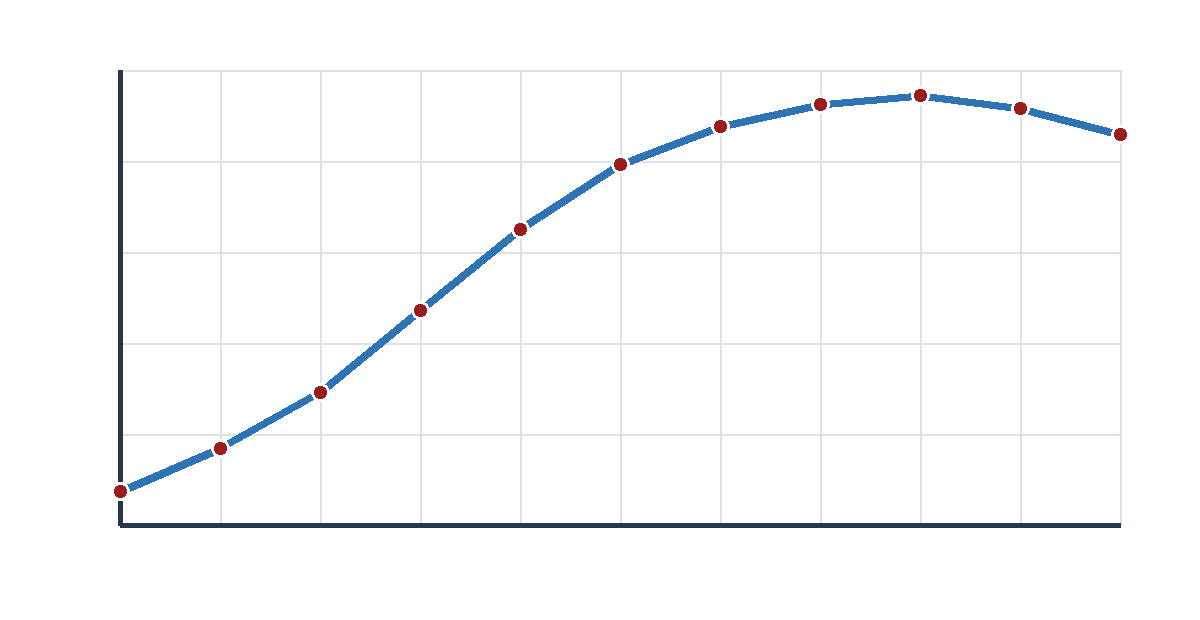
\includegraphics[width=0.72\linewidth]{assets/response-curve.png}
  \caption{Synthetic response curve / 合成响应曲线}
  \label{fig:response}
\end{figure}

Table~\ref{tab:metrics} contains small bilingual metrics.

\begin{table}[htbp]
  \centering
  \caption{Synthetic metrics / 合成指标}
  \label{tab:metrics}
  \begin{tabular}{lcc}
    \toprule
    Metric / 指标 & Baseline & Reviewed \\
    \midrule
    Peak response / 峰值 & 1.00 & 1.05 \\
    Residual ratio / 残余比 & 0.12 & 0.10 \\
    \bottomrule
  \end{tabular}
\end{table}

The bibliography entry is deliberately synthetic~\cite{fixture2026}.

\section{Conclusion / 结论}
\label{sec:conclusion}

The fixture closes by referring back to Section~\ref{sec:intro}. 该样例只用于
开源契约测试，不包含个人信息或未公开研究结果。
